% !TeX root = ./main.tex
\documentclass[10pt,conference]{IEEEtran}
\IEEEoverridecommandlockouts
% The preceding line is only needed to identify funding in the first footnote. If that is unneeded, please comment it out.
\usepackage{cite}
\usepackage{amsmath,amssymb,amsfonts}
\usepackage{algorithmic}
\usepackage{graphicx}
\DeclareGraphicsExtensions{.pdf,.png,.eps}
\usepackage{textcomp}
\usepackage{xcolor}
\usepackage[T1]{fontenc}

\usepackage{xspace}

\usepackage{multicol,lipsum}
\usepackage{multirow}

\def\BibTeX{{\rm B\kern-.05em{\sc i\kern-.025em b}\kern-.08em
    T\kern-.1667em\lower.7ex\hbox{E}\kern-.125emX}}

\begin{document}

\title{Categorizational Study on Commit Purpose For A Better Software Quality}

\author{
\IEEEauthorblockN{Jincheng He}
\IEEEauthorblockA{\textit{Department of Computer Science} \\
\textit{University of Southern California}\\
%City, Country \\
jinchenh@usc.edu}
}

\maketitle

\begin{abstract}
Developing software with the source code open to the public is very common; however, similar to its closed counterpart, open-source has quality problems, which cause functional failures, such as unsatisfying user experience, and non-functional, such as long responding time.
Previous researchers have revealed when, where, how and what the developers contribute to projects and how these aspects impact software quality. 
However, there has been little work on how different categories of commits impact software quality.
To improve the quality of open source software, we propose this research agenda to investigate how it is impacted by commits of different purposes.
By identifying these impacts, we will establish a new set of guidelines for commiting changes, thus improving the quality.

\end{abstract}

\begin{IEEEkeywords}
Software Engineering, Software Maintenance, Software Quality, Open Source Software
\end{IEEEkeywords}


\section{Introduction}

\subsection{TBD}

The length of commit messages (should be manually written?). Longer commit messages may imply higher software quality.
This research will focus on how different kinds of commits (represented by tags) impact the software quality metrics, including the commit messages and other metrics like security and vulnerability metrics.

\subsection{TBD}

What are the commit messages? We consider commit messages to be another kind of software quality metric. At the same time, it is used to convey the information of contributors of the commented revisions about what they did to the revision to others contributing to the projects, perhaps to other branches.


\section{Data}

To conduct this empirical study, we will need a sufficient data set from various open source projects.
The data set should contain the basic meta-data of projects and quality metrics reflecting the quality of those projects.
In this section, we will introduce our current data set and our plan to extend the data set.

\subsection{Current Data Set}
\label{sec:data}

The initial data set was introduced in previous studies \cite{pooyan_esem}, \cite{pooyan_qrs}. 
It includes data from 68 projects of Apache, Google, and Netflix and provides compilability information as well as software quality metrics of over 130000 commits, around 30000 out of which are considered as impactful commits, which are commits that developers change code in their core modules.

In addition, we manually tag 314 uncompilable commits and 1600 compilable commits, each of which are cross-validated by at least two different researchers.

\begin{figure}[htbp]
    \centerline{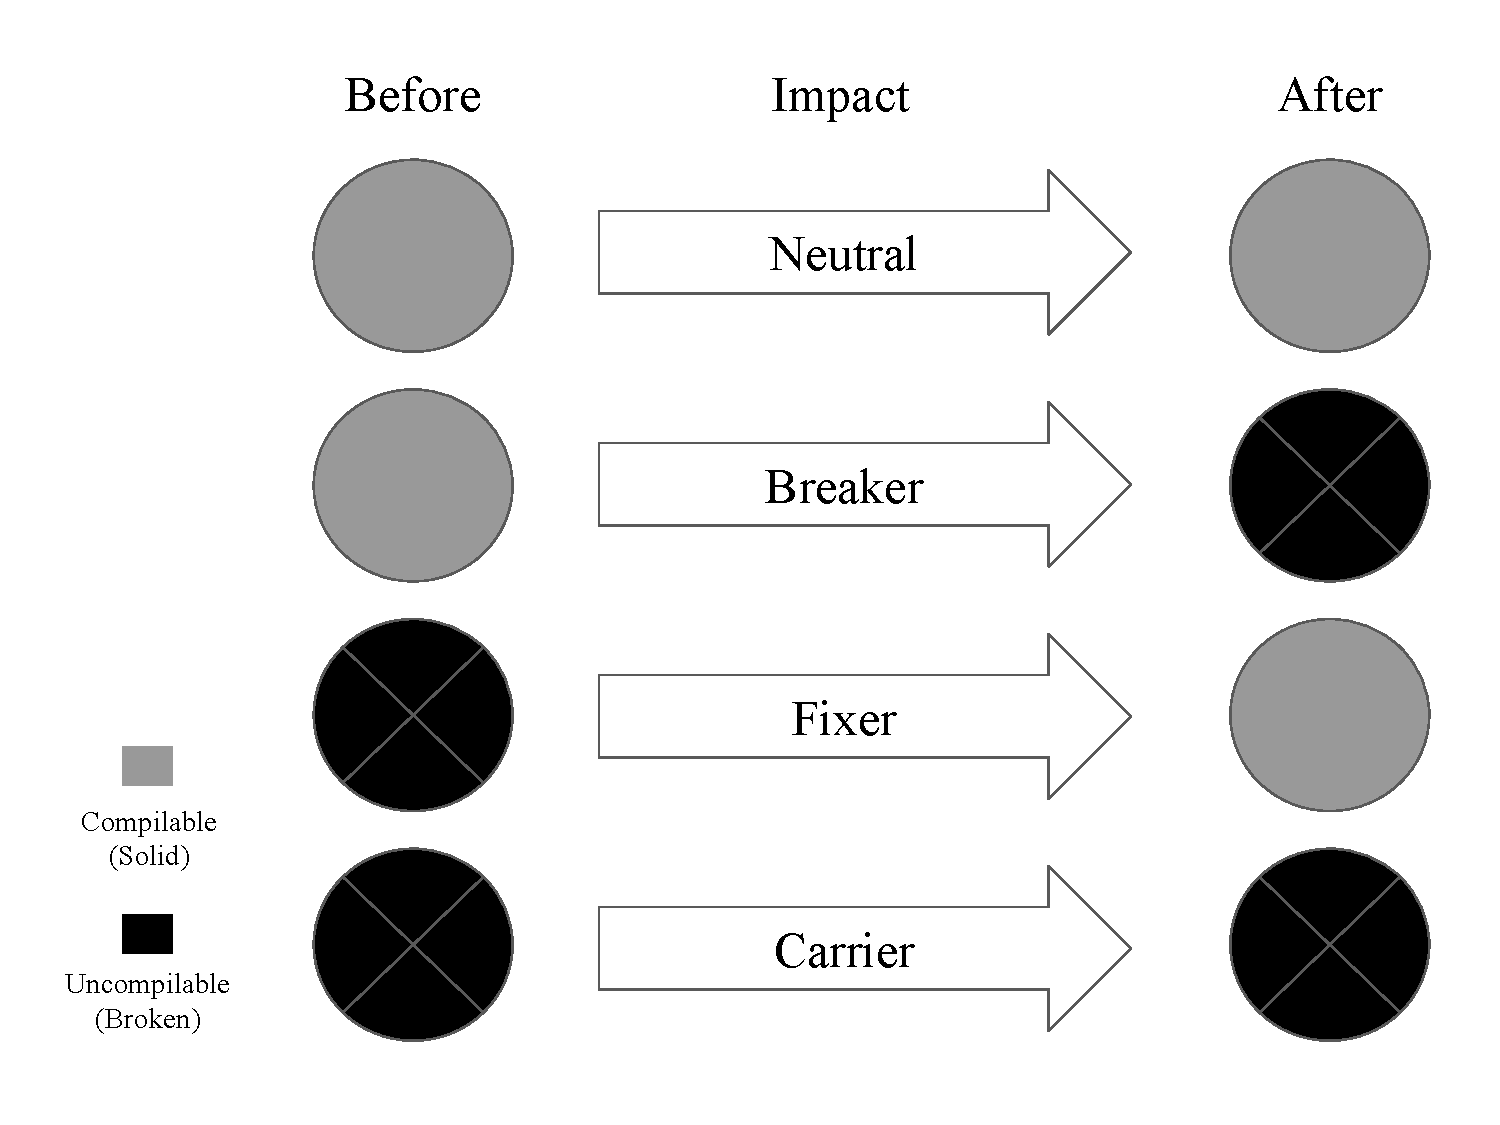
\includegraphics[scale=0.3]{figures/terminology.pdf}}
    \caption{Four Types of Impactful Commit}
    \label{fig:terminology}
    \end{figure}

We use the following terminology, as shown in Fig. \ref{fig:terminology}, to categorize commits based on their impact on compilability. 
As we consider one of the quality aspects is compilability, we also define all relevant terms.
%terms regarding it.

\begin{itemize}
\item A core module is a module that contains the majority of the source code, such as the main modules in most Apache library systems.
\item A commit is \textit{impactful} if it changes a core module.
An impactful commit is \textit{broken} if it creates an uncompilable revision; otherwise, it is \textit{solid}.
\item A broken commit is a \textit{breaker} if it breaks the compilability of its solid parent; otherwise, it is a \textit{carrier}.
\item A solid commit is a \textit{fixer} if it fixes its broken parent; otherwise it is \textit{neutral}.
Fig. \ref{fig:sequence} shows an example of a commit sequence with these four types of impactful commits.
\end{itemize}

\begin{figure}[htbp]
    \centerline{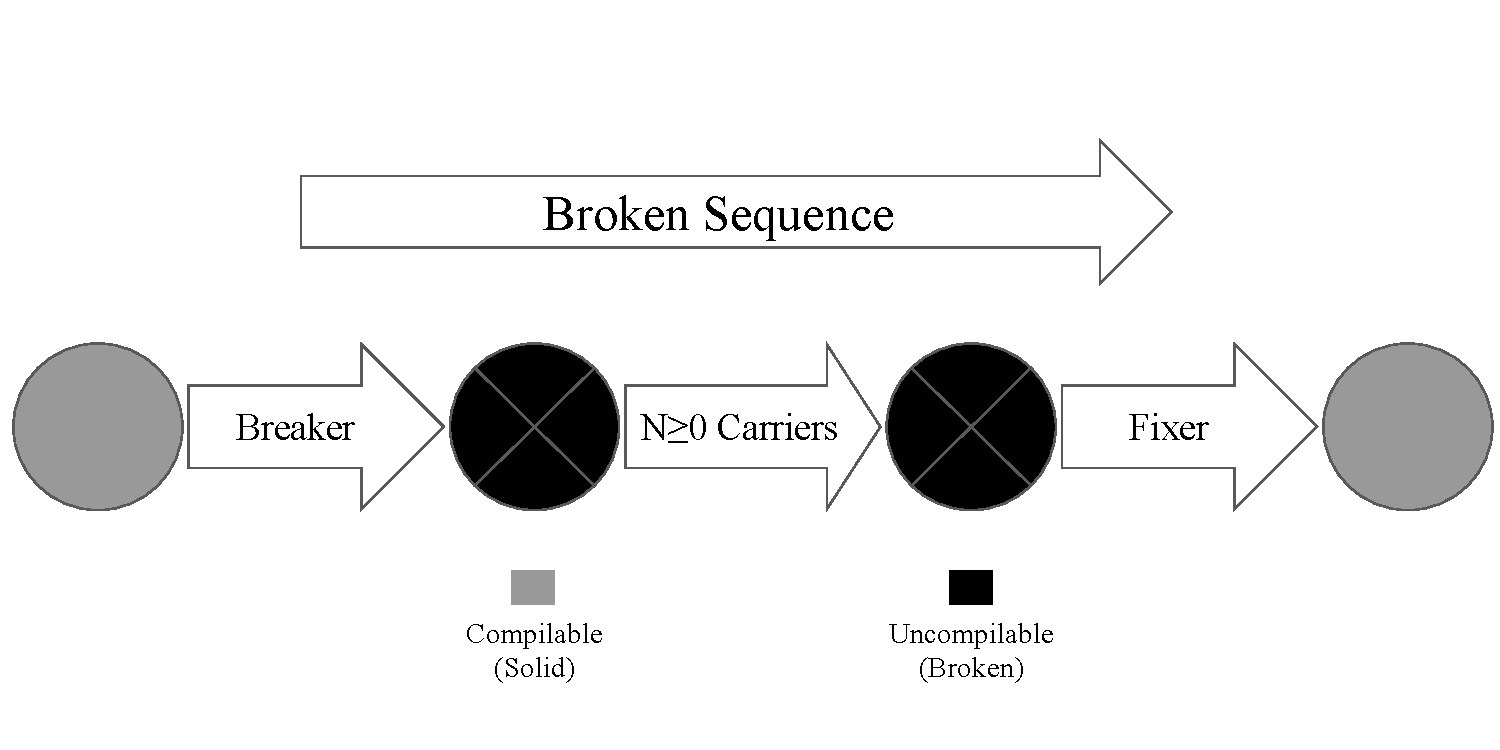
\includegraphics[scale=0.3]{figures/sequence.pdf}}
    \caption{An Example of a Broken Sequence}
    \label{fig:sequence}
    \end{figure}

We do not categorize orphan or merge commits into the aforementioned categories their impact is not identifiable by comparing two software revisions (i.e., before and after).

For selecting subject systems, we retrieve all Java projects owned by Google and Netflix from GitHub.
We select a system only if it 1) requires Ant, Maven, or Gradle for compilation and is not an Android, a Bazel, or an Eclipse project, 2) does not require manual installation of other tools (e.g., Protoc) for compilation, 3) is an official product of the organization, and 4) has a core module which contains a substantial amount of code.
We target the core module and identify ``impactfuls'' in each system and exclude those with fewer than 100 distinct revisions.
For selecting Apache subject systems, we use the same criteria as Netflix and Google, except that we only consider subject systems with fewer than 3000 commits by April 2017.

To develop the commit purpose taxonomy, we analyze 100 commits, using both the code and commit message in deriving the categorization. We consult with Hindle et al. to clarify category definitions and determine the categories included in our final taxonomy. 
In order to apply this taxonomy to small commits, we create further refinements of the definitions for four kinds of tasks. 

We use the resulting taxonomy to tag our dataset of 914 commits. Each commit is labelled and cross-validated by multiple individuals. 
Initial inconsistencies in tagging arise from ambiguities in the original taxonomy. 
To resolve these ambiguities, we study each inconsistent tag, identify the source of confusion and further refine the taxonomy definitions. 
The tag definitions are now more narrow in scope, and overlapping meaning between category definitions is reduced. 
This methodology ensures that our taxonomy can be applied consistently across varied tagging interpretations. 

We also define a threshold for identifying commit size, and use this to label each commit.
Some related works have introduced thresholds to differentiate between large and small commits; however, our dataset exhibits a more narrow range in commit size. 
The average commit size is also reduced due to our focus on the changes within a commit, as opposed to cumulative commit size. 
Thus, based on our dataset, we create a new threshold which defines commit size as the sum of added and deleted lines of code. The 314 uncompilable commits were split into two parts, with the smallest 157 commits labeled \textit{small}, and the remaining 157 labeled \textit{large}. 
The resulting threshold -- 184 lines of code -- is used to label the 600 compilable commits.
This threshold is based on the distribution of uncompilable commits in order to motivate discussion on the relative size and categorization of uncompilable commits. The final dataset contains 157 each of large and small uncompilable commits, and 138 \& 462 large and small compilable commits, respectively.

To analyze software quality evolution over uncompilable and compilable commits, we examine metrics on code complexity, maintainability, and security, provided by SonarQube\footnote{https://www.sonarqube.org/} and PMD\footnote{https://pmd.github.io/} and plan to utilize CAST\footnote{https://www.castsoftware.com/}. As uncompilable commits cannot be directly assessed by dynamic software quality analysis, we measure the overall quality change in the compilable commits before and after uncompilable sequences, extrapolating to determine the individual quality of each commit. 


\subsection{The Plan to Extend Current Data Set}

Choosing the data set is a critical issue for software repository mining research since, if the chosen data set is not representative, the conclusions will not be generally applicable.
To avoid this situation, we identify limitations of our current data set and how we plan to extend it as follows:
\begin{itemize}
    \item The current data set only contains projects from three large corporations, Google, Netflix and Apache. We plan to collect data from other corporations with different coding conventions.
    \item We focus on impactful commits in the current data set. To resolve this limitation, we plan to investigate non-impactful commits and evaluate whether it is necessary to extend this research to those commits.
\end{itemize}


\section*{4. Commit Types}
\subsection{Independent Change}
\label{sec:independent}

\begin{figure}[htbp]
\centerline{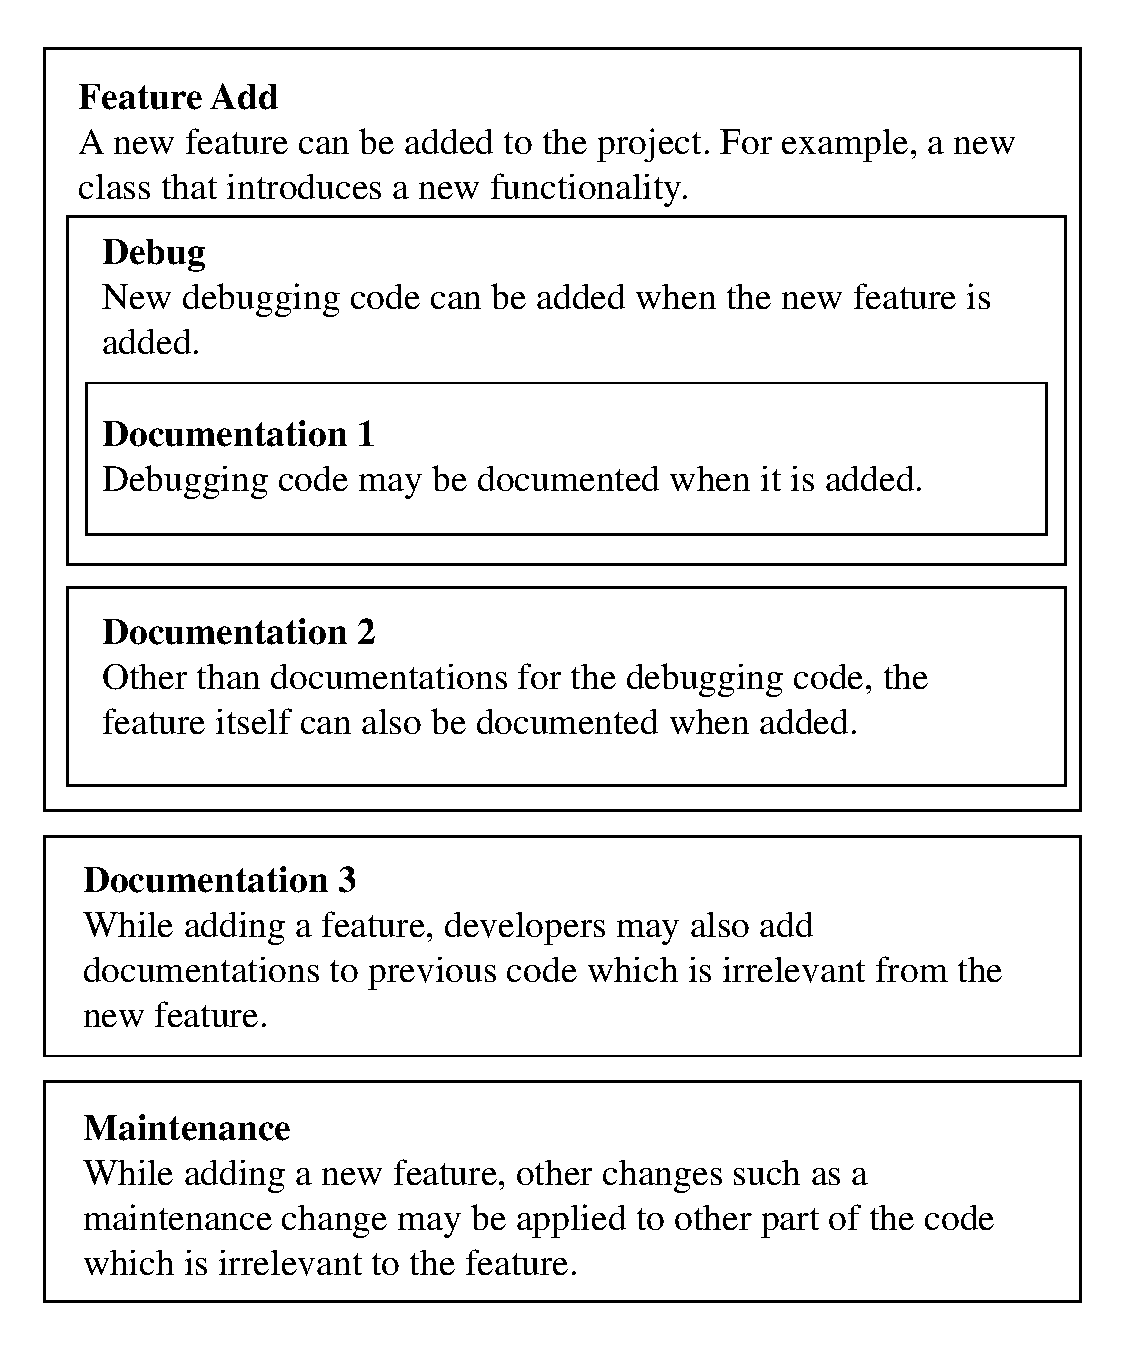
\includegraphics[scale=0.5]{figures/independent_change.pdf}}
\caption{Explanation For Independent Change}
\label{fig:Relationship}
\end{figure}

To improve our tagging, we first note that the original change type definitions overlap. For example, a documentation change may occur as part of a feature add commit. This increases tagging ambiguity and complexity, which we solve by introducing the concept of an \textit{independent change}.

We call a change an \textit{independent change} when it is not a part of other changes.
Fig. \ref{fig:Relationship} explains this concept. It illustrates a commit with multiple changes, in which a new feature contains three sub-changes.
Each block represents a code change. 
In the figure, a new feature change contains debugging code, documentation 1 for the functionality of the feature, documentation 2 for the debugging code, an irrelevant documentation 3, and an irrelevant maintenance change. 
In this case, the debugging code and documentation 1 and 2 are sub-changes to the new feature. 
As a result, we only assign a ``Feature Add'' tag to the new feature instead of assigning tags to all sub-changes. 
As documentation 3 and maintenance are both unrelated to the new feature, they will be assigned Documentation and Maintenance tags.
The new feature, documentation 3, and maintenance groups are independent changes, with the associated three independent tags forming a label the commit. 
With the introduction of independent change types, we reduce the ambiguity in the initial taxonomy which results in fewer cross-validation errors and improved tagging efficiency.

\subsection{Single-tagged Commit And Multi-tagged Commit}
When reviewing manual tagging, we analyze commits with different numbers of tags separately. 
The commits are divided into two groups: \textit{single-tagged} and \textit{multi-tagged}. \textit{Single-tagged} commits contain only one independent change, and \textit{multi-tagged} more than one. 

Fig. \ref{fig: cat_distribution} shows the tag-distributions of single and multi-tagged commits by commit purpose.
In the figure, black bars represent the rates when a certain commit is tagged a single category while gray bars are used to denote multi-tagged. For example, approximately 80\% commits are tagged Testing and more than 95\% of them are multi-tagged commits.
As shown in the figure, Build, Feature Add, Indentation, Refactoring, Testing arise more frequently in multi-tagged commits, indicating these tags tend to appear together with other tags. 
More than 95\% of testing commits have multiple tags, which is consistent with development practices of including the testing code along with most changes.
Documentation is more frequent in single-tagged commits, indicating that many documentation changes are added independently.
As the change of documentation is usually used to explain changed code, this may also imply that contributors often forget to add enough documentation when they accomplish a commit.
For other categories there are no apparent differences between single-tagged and multi-tagged commits.
In addition to comparing these two sets, we also study how many tags each commit has and its distribution. 
\begin{figure*}[htbp]
\centerline{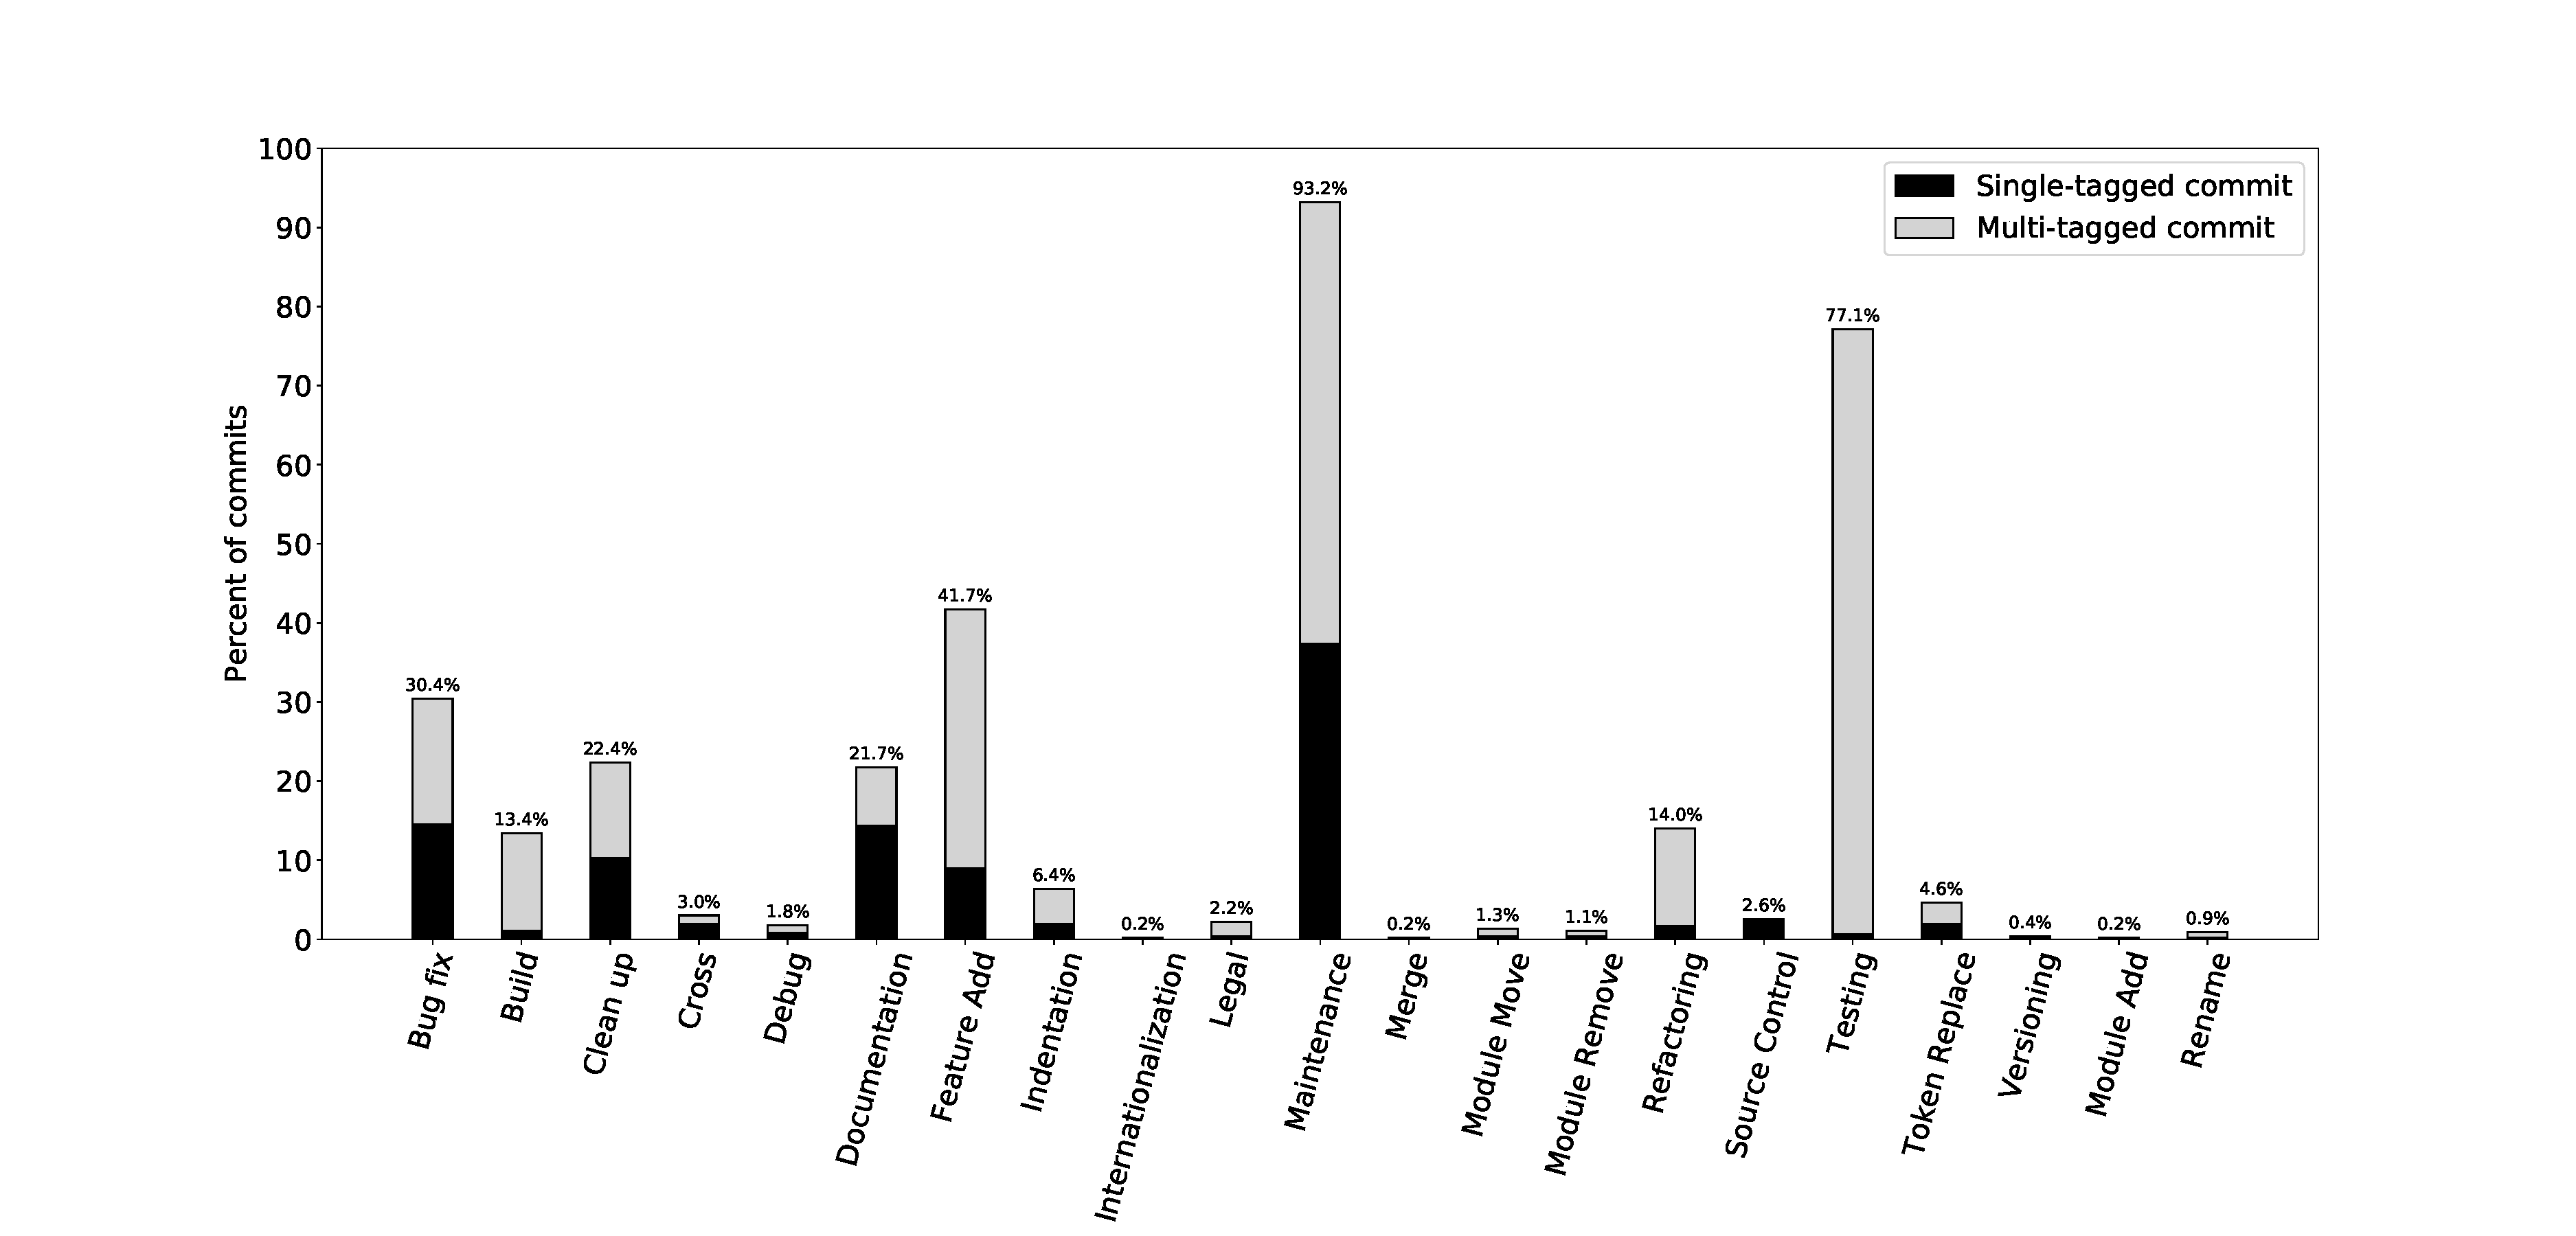
\includegraphics[scale=0.30]{figures/cat_distribution_over_s&m_commits.pdf}}
\caption{Change Type Distribution Between Single-tagged and Multi-tagged Commit}
\label{fig: cat_distribution}
\end{figure*}
\section{Software Quality}
\label{sec:quality}

The final goal of this research is to improve software quality.
Either the automation of the classification of commits or commit messages will in the end contribute to improved maintenance process, thus higher software quality.
In this section, we will introduce how we evaluate software quality in our research.

\subsection{Tool-based Quality Metrics}
Researchers use static analysis tools and other tools to assess the quality of software. 
For example, PMD, SonarQube and FindBugs give basic statistics of software, such as the lines of code, the number of functions, as well as quality-related metrics, such as vulnerability and code smell.
CAST software provide additional architecture evaluation.
We will evaluate software quality by using these metrics.

\subsection{Other Independently Defined Quality Aspects}
The software quality and quality metrics are not completely shown by the tools.
For example, they can't evaluate the quality when the software are not compilable. 
And the compilability is one of the most basic quality software should possess.

\subsubsection{Compilability}

A software revision created by a commit is expected to be compilable. However, uncompilability can occur due to careless development --- failure to compile the software locally prior to pushing to the shared repository. It can also result from variations in build environments, incompatibility across overlapping changes made by multiple developers, or changes in upstream dependencies. 
The presence of compile errors inhibits bytecode and dynamic software analysis, as well as static analysis when the code is unparsable \cite{pooyan_esem}.
Previous studies \cite{pooyan_esem, 8170083, Hassan2017ESEM, SMR:SMR1838} have shown that even in popular open-source projects maintained by major software organizations, build-breaking commits can occur.

Behnamghader et al. \cite{pooyan_qrs} explore the qualitative properties of uncompilable commits.
Further insight into the types of commits that most frequently cause build errors can help to inform better development practices. Additionally, this correlation can be used as a part of future methods for predicting and preventing uncompilable commits. 
Analyzing the degradation of software quality over multiple uncompilable commits highlights the long-term negative impact of careless development, and the importance of fixing build errors immediately after they take place.
Also, understanding the purposes of those uncompilable commits can result in preparing guidelines to avoid such degradation in the future.

Multiple recent studies \cite{8170083,Seo:2014:PBE:2568225.2568255,Hassan2017ESEM,macho2018automatically,SMR:SMR1838, pooyan_esem, pooyan_qrs} have assessed the compilability of software repositories. 
To our knowledge, none address the effects of developer purpose on uncompilability, or how software quality evolves when the code is uncompilable. 
Hassan et al. \cite{8170083} focus on automatically building the last commit for the top 200 Java repositories on GitHub.
Seo et al. \cite{Seo:2014:PBE:2568225.2568255} analyze 26.6 million builds produced over a period of 9 months by Google engineers, reporting the build failure frequency and cause, as well as how long it takes to remediate.
Hassan et al. \cite{Hassan2017ESEM} propose a build-outcome prediction model, based on combined features of build-instance metadata and code changes, to predict whether a build will be successful.
Macho et al. \cite{macho2018automatically} identify 125 commits in 23 repositories that repair a missing dependency, qualitatively and quantitatively analyze how the fix is applied, and propose an approach to fix dependency build breakage automatically.
Tufano et al. \cite{SMR:SMR1838} study the compilability of 219,395 snapshots of 100 Java projects from the Apache Foundation, analyzing the frequency and possible causes of broken snapshots.
Benamghader et al. \cite{pooyan_qrs} qualitatively study why developers commit uncompilable code, and design an approach \cite{pooyan_esem} to increase compilation ratio over commit history and to study sequences of uncompilable commits in terms of their length and interval.

To understand how software quality evolves over uncompilability, we identify all the broken sequences in our dataset.
Each broken sequence starts with a breaker and ends with a fixer. The broken commits in the sequence cannot be analyzed using software quality tools. 
However, we can compare software quality between two revisions to understand how software quality evolves over the sequence: the revision produced by the impact-parent of the breaker and the one produced by the fixer.
The former is the last solid revision before the sequence begins and the latter is the first solid revision after the sequence ends. 

\subsection{Our Approach}

In our research, we will combine the quality metrics with other quality aspects, such as compilability to reflect the overall quality of the software.
We will investigate how different categories of changes impact the quality and how we can avoid the defects.

\section{Commit Message}
\subsection{Initiatives of Commit Messages}
\subsection{Preprocessing Removal of Useless Information in Commit Messages}
\subsection{The Relation Between Commit Message and Software Quality}
\section{Code Patterns}
\subsection{Different Patterns Existing in Code.}
\subsection{Different Patterns May Have Different Impact on Software Quality}
\section*{7. Conclusions}
\section*{Acknowledgment}
\label{sec:acknowledgment}
This material is based upon work supported in part by the U.S. Department of Defense through the Systems Engineering Research Center (SERC) under Contract No. HQ0034-13-D-0004 Research Task WRT 1016 -- ``Reducing Total Ownership Cost (TOC) and Schedule.'' SERC is a federally funded University Affiliated Research Center managed by Stevens Institute of Technology. 



\medskip
\bibliographystyle{./bibliography/IEEEtran}
\bibliography{./bibliography/IEEEabrv,./bibliography/IEEEexample,./bibliography/references}

\vspace{12pt}
\color{red}
%IEEE conference templates contain guidance text for composing and formatting conference papers. Please ensure that all template text is removed from your conference paper prior to submission to the conference. Failure to remove the template text from your paper may result in your paper not being published.


\end{document}